\documentclass[10pt,a4paper]{article}
\usepackage[top=1.4cm, bottom=1.4cm, left=1.6cm, right=1.6cm, headheight=14pt, footskip=18pt]{geometry}
\usepackage[utf8]{inputenc}
\usepackage{amsmath,amsfonts,amssymb}
\usepackage{graphicx}
\usepackage{tikz}
\usepackage{circuitikz}
\usetikzlibrary{calc,patterns}
\usepackage[most]{tcolorbox}
\usepackage{enumitem}
\usepackage{fancyhdr}
\usepackage{booktabs}
\usepackage{tabularx}
\usepackage{colortbl}
\usepackage{hyperref}

% --- Palet Warna Resmi UNIB ---
\definecolor{unibblue}{RGB}{0, 32, 96}
\definecolor{unibgold}{RGB}{197, 160, 89}
\definecolor{unibgreen}{RGB}{34, 112, 60}
\definecolor{boxbg}{RGB}{248, 250, 253}
\definecolor{linegray}{RGB}{210, 215, 225}

% --- Pengaturan Header & Footer ---
\pagestyle{fancy}
\fancyhf{}
\lhead{\footnotesize\textbf{\color{unibblue}Universitas Bengkulu} \textbar\ Program Studi S1 Teknik Elektro}
\rhead{\footnotesize\color{gray}Persamaan Diferensial (Genap 2026)}
\lfoot{\footnotesize\color{gray}Problem Set OBE \textbar\ \textbf{Video}: \url{https://youtu.be/J4XziBcVtfk} \textbar\ \href{https://www.youtube.com/playlist?list=PLS5oOZWXZeTw}{\color{unibblue}\textbf{Playlist}}}
\cfoot{\footnotesize\color{gray}Hal. \thepage\ dari 2}
\rfoot{\footnotesize\color{unibblue}\textbf{Minggu 15: Polinomial Legendre \& Persamaan ...}}
\renewcommand{\headrulewidth}{0.6pt}
\renewcommand{\footrulewidth}{0.4pt}

\begin{document}

% ==================== HALAMAN 1 ====================
\noindent\begin{minipage}[c]{0.68\textwidth}%
  {\large\textbf{\color{unibblue}PROBLEM SET (TUGAS MANDIRI TERSTRUKTUR)}}\\[1mm]
  {\normalsize\textbf{Mata Kuliah: Persamaan Diferensial (2 SKS)}}\\[0.5mm]
  {\small\textbf{Topik Minggu 15:} Polinomial Legendre \& Persamaan Gelombang Elektromagnetik}%
\end{minipage}%
\hfill%
\begin{minipage}[c]{0.30\textwidth}%
  \begin{tcolorbox}[colback=unibblue!5,colframe=unibblue,boxrule=0.6pt,arc=2pt,left=4pt,right=4pt,top=2pt,bottom=2pt]
    \scriptsize
    \textbf{Nama:} \dotfill\\[1.2mm]
    \textbf{NPM:} \dotfill\\[1.2mm]
    \textbf{Kelas/Klp:} \dotfill\\[1.2mm]
    \textbf{Nilai Final:} \hfill \textbf{/ 100}
  \end{tcolorbox}%
\end{minipage}\par

\vspace{1.5mm}

% Kotak Sub-CPMK & Pedoman Tugas Terstruktur
\begin{tcolorbox}[colback=boxbg,colframe=unibgold!90!black,boxrule=0.6pt,arc=2pt,left=5pt,right=5pt,top=3pt,bottom=3pt,title=\textbf{\scriptsize Capaian Pembelajaran (Sub-CPMK 6) \& Pedoman Pengerjaan Tugas}]
  \scriptsize
  \textbf{Sub-CPMK 6:} Mahasiswa mampu memecahkan Persamaan Diferensial Legendre dalam koordinat bola serta menurunkan formulasi Persamaan Gelombang Elektromagnetik Helmholtz dari 4 Persamaan Maxwell.\\
  \textbf{Video Perkuliahan (YouTube):} \url{https://youtu.be/J4XziBcVtfk} \hfill \textbf{Playlist:} \href{https://www.youtube.com/playlist?list=PLS5oOZWXZeTw}{\color{unibblue}\textbf{bit.ly/pd-unib-playlist}}\\\textbf{Ketentuan Tugas:} Kerjakan secara mandiri pada kertas folio/A4 bergaris atau laporan digital rapi. Lampirkan penurunan rumus analitis lengkap dan cetak visualisasi kode program Julia (Soal C6). Kumpulkan pada awal perkuliahan minggu berikutnya.
\end{tcolorbox}

\vspace{1.5mm}

\noindent{\textbf{\color{unibblue}\large BAGIAN I: FONDASI KONSEPTUAL \& PENURUNAN MATEMATIS}}\par
\vspace{1mm}

% Soal C1
\noindent\textbf{1. (C1 - Mengingat \textbar\ Bobot: 10 Poin)}\par\vspace{0.8mm}
{\footnotesize Tuliskan bentuk baku Persamaan Diferensial Legendre $(1 - x^2) \frac{d^2 y}{dx^2} - 2x \frac{dy}{dx} + n(n+1)y = 0$, dan sebutkan polinomial Legendre untuk tiga derajat pertama: $P_0(x)$, $P_1(x)$, dan $P_2(x)$.}\par

\vspace{2.5mm}

% Soal C2
\noindent\textbf{2. (C2 - Memahami \textbar\ Bobot: 15 Poin)}\par\vspace{0.8mm}
{\footnotesize Jelaskan sifat ortogonalitas Polinomial Legendre $\int_{-1}^1 P_m(x) P_n(x) dx = \frac{2}{2n+1} \delta_{mn}$. Bagaimana sifat ini dimanfaatkan untuk mengevaluasi koefisien ekspansi deret potensial elektrostatika pada sistem dengan simetri bola?}\par

\vspace{2.5mm}

% Soal C3
\noindent\textbf{3. (C3 - Menerapkan \textbar\ Bobot: 20 Poin)}\par\vspace{0.8mm}
\noindent\begin{minipage}[t]{0.60\textwidth}%
  {\footnotesize Sebuah bola konduktor netral beradius $a = 15\text{ cm}$ diletakkan di dalam medan listrik luar yang seragam $\vec{E}_0 = E_0 \hat{a}_z$ ($E_0 = 50\text{ kV/m}$). Distribusi potensial di luar bola memenuhi persamaan Laplace koordinat bola dengan solusi umum $V(r,\theta) = \sum_{n=0}^\infty (A_n r^n + B_n r^{-(n+1)}) P_n(\cos\theta)$. Tentukan fungsi analitis potensial $V(r,\theta)$ secara tuntas!}%
\end{minipage}%
\hfill%
\begin{minipage}[t]{0.37\textwidth}%
  \centering
  \resizebox{0.95\linewidth}{!}{%
  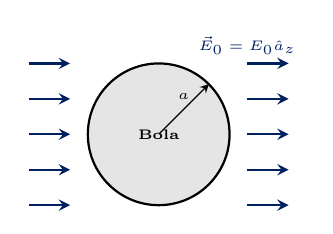
\begin{tikzpicture}[scale=0.75]
    \draw[thick, fill=gray!20] (0,0) circle (1.2);
    \draw[->, >=stealth] (0,0) -- (0.85,0.85) node[midway, above, font=\tiny] {$a$};
    \node at (0,0) [font=\tiny\bfseries] {Bola};
    \foreach \y in {-1.2, -0.6, 0, 0.6, 1.2} {
      \draw[->, >=stealth, thick, unibblue] (-2.2,\y) -- (-1.5,\y);
      \draw[->, >=stealth, thick, unibblue] (1.5,\y) -- (2.2,\y);
    }
    \node at (1.5,1.5) [font=\tiny\bfseries, unibblue] {$\vec{E}_0 = E_0 \hat{a}_z$};
  \end{tikzpicture}%
  }%
\end{minipage}\par

\vfill

% Kotak Formula Rujukan Teknis & Standar Industri
\begin{tcolorbox}[colback=unibblue!3,colframe=unibblue,colbacktitle=unibblue,coltitle=white,boxrule=0.6pt,arc=2pt,left=6pt,right=6pt,top=3pt,bottom=3pt,title=\textbf{\scriptsize FORMULA RUJUKAN TEKNIS \& STANDAR INDUSTRI TERKAIT}]
  \scriptsize
  \begin{itemize}[leftmargin=*, nosep]
  \item Persamaan Diferensial Legendre Orde $n$: $(1-x^2) \frac{d^2 y}{dx^2} - 2x \frac{dy}{dx} + n(n+1) y = 0$
  \item Polinomial Legendre: $P_0(x) = 1$, $P_1(x) = x$, $P_2(x) = \frac{1}{2}(3x^2 - 1)$, $P_3(x) = \frac{1}{2}(5x^3 - 3x)$
  \item Solusi Potensial Bola Konduktor: $V(r,\theta) = \sum_{n=0}^\infty \left( A_n r^n + \frac{B_n}{r^{n+1}} \right) P_n(\cos\theta)$
  \item Vektor Medan Listrik Koordinat Bola: $E_r = -\frac{\partial V}{\partial r}$, $E_\theta = -\frac{1}{r}\frac{\partial V}{\partial \theta}$, $E_\phi = -\frac{1}{r\sin\theta}\frac{\partial V}{\partial \phi}$
\end{itemize}
\end{tcolorbox}

\newpage
% ==================== HALAMAN 2 ====================

\noindent{\textbf{\color{unibblue}\large BAGIAN II: ANALISIS SISTEM, EVALUASI STANDAR, \& KOMPUTASI JULIA}}\par
\vspace{1mm}

% Soal C4
\noindent\textbf{4. (C4 - Menganalisis \textbar\ Bobot: 20 Poin)}\par\vspace{0.8mm}
{\footnotesize Analisis Penurunan Persamaan Gelombang Elektromagnetik 3D: Terapkan operator rotasi $\nabla \times (\nabla \times \vec{E})$ pada Hukum Faraday $\nabla \times \vec{E} = -\frac{\partial \vec{B}}{\partial t}$ di ruang bebas tanpa muatan dan arus ($\rho=0, \vec{J}=0$). Gunakan identitas vektor $\nabla \times (\nabla \times \vec{E}) = \nabla(\nabla \cdot \vec{E}) - \nabla^2 \vec{E}$ untuk membuktikan bahwa medan listrik memenuhi persamaan gelombang 3D dengan kecepatan rambat $c = 1/\sqrt{\mu_0 \epsilon_0} \approx 3 \times 10^8\text{ m/s}$.}\par

\vspace{3.5mm}

% Soal C5
\noindent\textbf{5. (C5 - Mengevaluasi \textbar\ Bobot: 20 Poin)}\par\vspace{0.8mm}
{\footnotesize Evaluasi Vektor Poynting $\vec{S} = \vec{E} \times \vec{H}$ dan Batas Paparan Publik \textbf{IEEE Std C95.1}: Gelombang elektromagnetik transversal (TEM) memiliki amplitudo medan listrik $E = 50\text{ V/m}$ di bawah koridor saluran transmisi SUTET 500 kV PLN. (a) Hitung magnitudo medan magnetik $H = E/\eta_0$ di mana impedansi ruang bebas $\eta_0 = \sqrt{\mu_0/\epsilon_0} \approx 377\,\Omega$; (b) Hitung densitas fluks daya rata-rata $S_{\text{avg}} = \frac{1}{2} E H$; (c) Evaluasi apakah nilai radiasi daya tersebut aman bagi masyarakat sekitar.}\par

\vspace{3.5mm}

% Soal C6
\noindent\textbf{6. (C6 - Merancang \& Komputasi Julia \textbar\ Bobot: 15 Poin)}\par\vspace{0.8mm}
{\footnotesize Rancang skrip program ilmiah berbasis \textbf{Julia} menggunakan pustaka \texttt{Plots.jl} untuk memetakan garis-garis gaya medan listrik ekuipotensial dipol bola hasil penurunan Soal 3. Program harus menghitung vektor medan radial $E_r = -\frac{\partial V}{\partial r}$ dan transversal $E_\theta = -\frac{1}{r}\frac{\partial V}{\partial \theta}$ serta menampilkan grafik vektor medan (*quiver plot*) di sekitar bola konduktor.}\par

\vfill

% Tabel Rekapitulasi Skor OBE & Lembar Catatan Umpan Balik Dosen
\noindent\begin{minipage}[b]{0.62\textwidth}%
  \centering
  \scriptsize
  \begin{tabular}{|c|c|c|c|c|c|c|}
    \hline
    \rowcolor{unibblue}
    \textbf{\color{white}C1} & \textbf{\color{white}C2} & \textbf{\color{white}C3} & \textbf{\color{white}C4} & \textbf{\color{white}C5} & \textbf{\color{white}C6} & \textbf{\color{white}Total} \\
    \rowcolor{unibblue!10}
    10 Pts & 15 Pts & 20 Pts & 20 Pts & 20 Pts & 15 Pts & 100 Pts \\
    \hline
    & & & & & & \\[3mm]
    \hline
  \end{tabular}%
\end{minipage}%
\hfill%
\begin{minipage}[b]{0.35\textwidth}%
  \centering
  \scriptsize
  \textbf{Verifikasi Dosen / Asisten:}\\[6mm]
  (\dotfill)\\[1mm]
  \tiny Tanggal: \dotfill
\end{minipage}\par

\vspace{2mm}
\begin{tcolorbox}[colback=white,colframe=unibblue!40!black,colbacktitle=unibblue!10,coltitle=unibblue,boxrule=0.5pt,arc=2pt,left=5pt,right=5pt,top=3pt,bottom=3pt,title=\textbf{\tiny Catatan Evaluasi \& Umpan Balik Dosen Pengampu}]
  \tiny
  \textbf{Rubrik Pemeriksaan Pengerjaan Tugas Mandiri:}\par\vspace{0.8mm}
  $\square$ Penurunan matematis langkah-demi-langkah runtut (C1--C4) \hfill $\square$ Validasi analitis \& standar industri IEEE/IEC/SPLN akurat (C5)\\[0.8mm]
  $\square$ Skrip program Julia mandiri \& grafik visualisasi terlampir (C6) \hfill $\square$ Kerapian format laporan \& ketepatan waktu pengumpulan\\[2.0mm]
  \textbf{Catatan / Koreksi Khusus Dosen:}\\[1.6cm]
\end{tcolorbox}

\end{document}
